
\chapter{Electrical activity in the brain}

The aim of this chapter is to describe the biology of the brain, discuss how brain activity can be measured and where the measurable activity originates from. The chapter will also compare different techniques and devices used to measure brain activity and finally suitable device for controlling a robot is chosen.

\section{Source of the electrical activity}
\label{sec:neuron}

As all living organisms are composed of cells, so are humans and the human brain. The brain consists of nerve cells called \glspl{neuron} and non-neural cells. There are approximately 86 billion \glspl{neuron} in the human brain and roughly as much non-neural cells~\cite{neuroncount}. The aim of this section is to describe how \glspl{neuron} interact with each other and discuss what aspect of this communication can be measured.

\begin{figure}[b!]
	\centering
	\begin{subfigure}{0.48\textwidth}
		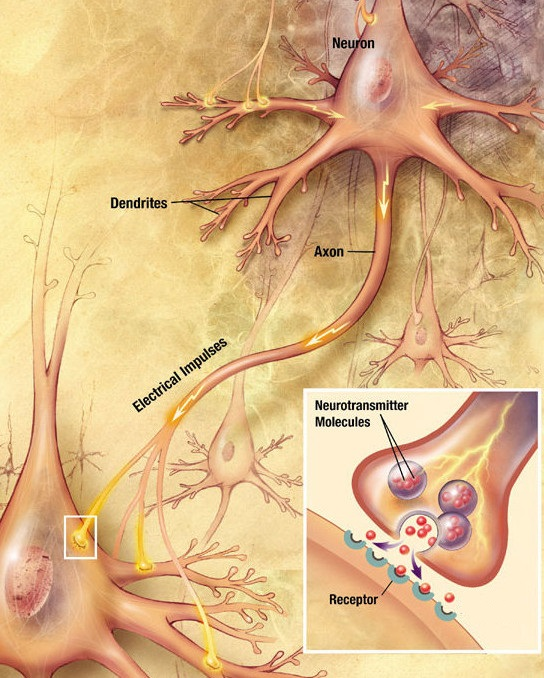
\includegraphics[width=\textwidth]{synapse_modified.jpg}
		\caption{Neurons and a chemical synapse~\cite[p.~17]{neuronpic}}
		\label{fig:neuron_synapse}
	\end{subfigure}
	~
	\begin{subfigure}{0.48\textwidth}
		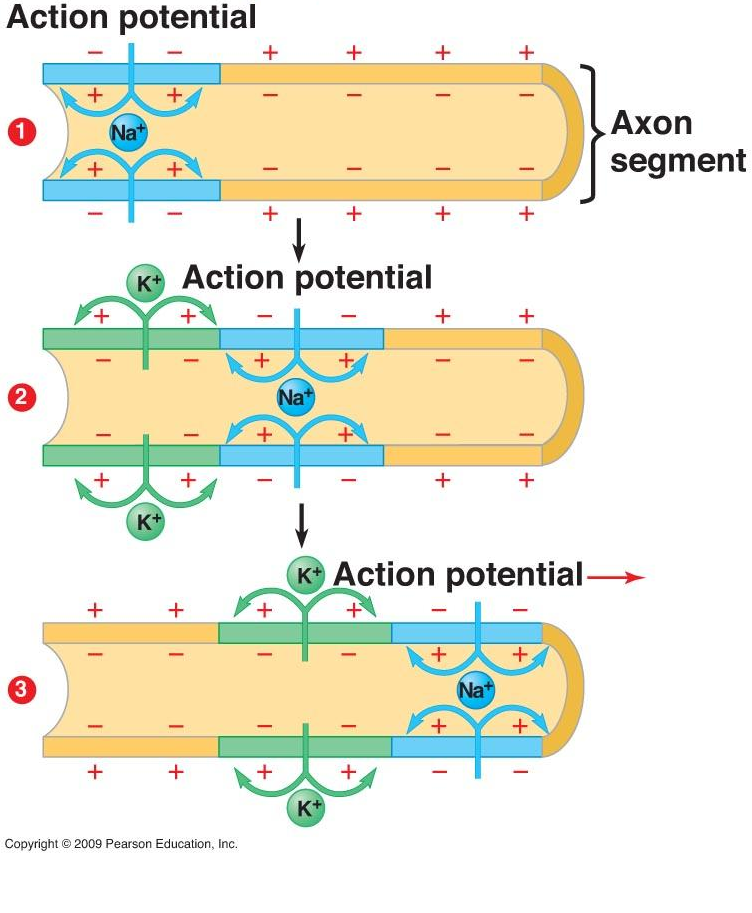
\includegraphics[width=\textwidth]{action_potential.png}
		\caption{Action potential~\cite{action_potential_pic}}
		\label{fig:action_potential}
	\end{subfigure}
	\caption{The structure of a neuron}
\end{figure}

A typical \gls{neuron} has a cell body, multiple nerve endings or \glspl{dendrite}, and one nerve fibre or \gls{axon}. Both \glspl{dendrite} and \glspl{axon} can branch multiple times. \Glspl{neuron} interact with each other via electro-chemical signals that are transmitted through various connections. These connections are not static and can change over time. The connection between an \gls{axon} and a \gls{dendrite} is called a \gls{synapse}. See figure~\ref{fig:neuron_synapse} for an example of \glspl{neuron} and a \gls{synapse}. The general rule is that a \gls{neuron} sends signals through its \gls{axon} and receives signals through \glspl{dendrite}. Functionally related \glspl{neuron} are connected to each other and form \glspl{neural pathway}~\cite{neuralpathway}.

To send signals, \glspl{neuron} must be able to maintain electric potential called \gls{membrane potential}. \Gls{membrane potential} is the difference in electric potential between the interior and the exterior of a cell. When a \gls{neuron} is not sending signals or in other words, when neuron is at a \gls{resting state}, its \gls{membrane potential} is slightly negative. The \gls{membrane potential} of a \gls{neuron} at a \gls{resting state} is called \gls{resting potential}. Negative \gls{resting potential} is achieved by having more positively charged ions around the cell than inside the cell.

By having stable \gls{resting potential}, \glspl{neuron} are able to send signals by rapidly increasing and decreasing the \gls{membrane potential} along an \gls{axon}. This event is called an \gls{action potential}. See figure~\ref{fig:action_potential} for example. To increase or decrease the \gls{membrane potential} of a cell, \glspl{ionophoric protein} are used. These proteins transport ions across the cell membrane to regulate the concentration of ions inside the cell. Since ions are electrically charged, the concentration of ions inside a cell affects the \gls{membrane potential} of the cell. The \gls{membrane potential} of a cell can be increased by transporting positive ions into the cell and decreased by transporting positive ions out of the cell. 

An \gls{action potential} or signal sending is initiated when the \gls{membrane potential} of a \gls{neuron} exceeds certain threshold value called \gls{threshold potential}. The \gls{membrane potential} of a \gls{neuron} can increase when the \gls{neuron} receives signals from other \glspl{neuron}. The \gls{neuron} that receives a signal is called \gls{postsynaptic cell}. The received signal can cause the \gls{membrane potential} of the \gls{postsynaptic cell} to increase or decrease. This change in \gls{membrane potential} is called a \gls{postsynaptic potential}. If the \gls{postsynaptic potential} is large enough for the \gls{membrane potential} to exceed \gls{threshold potential}, an \gls{action potential} is initiated in the \gls{postsynaptic cell}.

The following paragraph is mainly based on the article by Buzsaki \textit{et al.}~\cite{electric_field}. The \gls{postsynaptic potential} is caused by ions flowing into the cell. To achieve electroneutrality, a balancing flow of ions from the interior to the exterior of the cell is needed. The ions of the balancing flow have the same electric charge as the entering ions. If the ions flowing into the cell have
\begin{itemize}
	\item positive charge, then 
	\subitem the \gls{membrane potential} of the cell increases;
	\subitem location where positive ions enter the cell is called a \gls{sink};
	\subitem location where positive ions exit the cell is called a \gls{source}; and
	\subitem as a result, there are less positive ions around \gls{sink} and more around \gls{source};
	\item negative charge, then
	\subitem the \gls{membrane potential} of the cell decreases;
	\subitem location where negative ions enter the cell is called a \gls{source};
	\subitem location where negative ions exit the cell is called a \gls{sink}; and
	\subitem as a result, there are less negative ions around \gls{source} and more around \gls{sink}.
\end{itemize}

In both cases, the \gls{source} has more positive electrical charge than the \gls{sink}. Since the \gls{source} and the \gls{sink} have different electric potentials, they form a \gls{current dipole}. See figure~\ref{fig:dipole} for illustration.

\begin{figure}[h!]
	\centering
	\begin{subfigure}{0.48\textwidth}
		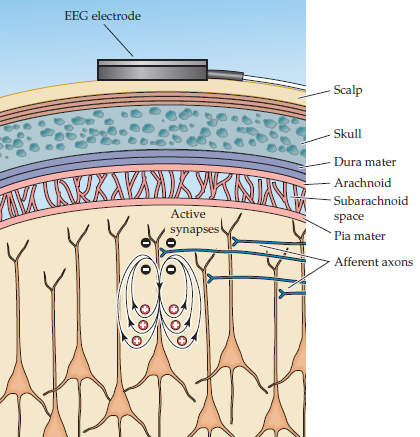
\includegraphics[width=\textwidth]{dipole_neuron.png}
		\caption{Current dipole generated by a neuron~\cite[p.~669]{neuroscience}}
		\label{fig:dipole_neuron}
	\end{subfigure}
	~
	\begin{subfigure}{0.48\textwidth}
		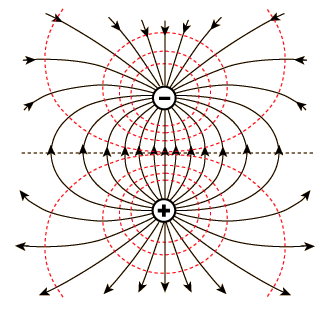
\includegraphics[width=\textwidth]{dipole_electric.png}
		\caption{The electric field of an electric dipole\protect\footnotemark}
		\label{fig:dipole_electric}
	\end{subfigure}
	\caption{Dipoles}
	\label{fig:dipole}
\end{figure}
\footnotetext{http://hyperphysics.phy-astr.gsu.edu/hbase/electric/equipot.html}

\Glspl{current dipole} are important because it is possible to measure the electric field produced by these \glspl{current dipole} from the scalp. See figure~\ref{fig:dipole_neuron} for illustration. Measuring these electric fields is further discussed in section~\ref{sec:EEG}. Although \glspl{action potential} generate stronger currents than \glspl{postsynaptic potential}, their duration is short and nearby \glspl{neuron} rarely fire synchronously~\cite{electric_field}. Thus recording the electrical activity of the brain mainly relies on the electric fields of the \glspl{current dipole} generated by \glspl{neuron}.

\section{Functional neuroimaging methods}
\label{sec:neuroimaging}

As discussed in section~\ref{sec:neuron}, \glspl{neuron} in the brain are sending electrochemical signals to communicate with each other. There are several techniques available to measure this activity. The aim of this section is to briefly compare various non-invasive techniques. Measuring an aspect of brain function is called \gls{functional neuroimaging} and common measurement methods divide into \gls{haemodynamic} and \gls{electromagnetic} techniques.

\Gls{haemodynamic} techniques measure blood oxygenation and blood flow in the brain. More oxygen has to be delivered to more active brain regions and this allows the brain activity to be measured. \Gls{haemodynamic} techniques include \gls{fMRI}, \gls{fNIRS} and \gls{PET}.

\Gls{electromagnetic} techniques measure either electrical activity or magnetic fields produced by the electrical activity along the scalp. \Gls{electromagnetic} techniques include \gls{EEG} and \gls{MEG}. These methods have lower \gls{temporal resolution} than \gls{haemodynamic} methods, but measure only the activity in the outer layer of the brain. \Gls{temporal resolution} is the smallest time period of neural activity that is reliably separated out by measuring technique.

To decide which method is best for controlling a robot, cost, portability and \gls{temporal resolution} of each method is compared. See table~\ref{tab:neuroimaging} for details. For real-time robot controlling, lower \gls{temporal resolution} is better because it enables faster decision making.

% Constants for table

\newcommand{\pMEG}{\tablefootnote{http://neurogadget.com/2012/12/15/inexpensive-magnetoencephalography-meg-system-could-be-available-at-every-hospital/6495}}
\newcommand{\pfMRI}{\tablefootnote{http://info.blockimaging.com/bid/92623/MRI-Machine-Cost-and-Price-Guide}}
\newcommand{\pPET}{\tablefootnote{http://info.blockimaging.com/bid/68875/How-Much-Does-a-PET-CT-Scanner-Cost}}
\newcommand{\pEEG}{\tablefootnote{http://en.wikipedia.org/wiki/Comparison\_of\_consumer\_brain-computer\_interfaces}}
\newcommand{\pNIRS}{\cite{NIRS}}
\newcommand{\tresol}{\cite{timeresol}}

% Table

\begin{table}[h]
	\centering
	\begin{tabular}{|c|c|c|c|c|c|}\hline
			& Price	from				& Portable	& Temporal resolution		& Special requirements			\\\hline
\gls{MEG}	& millions\pMEG				& no		& milliseconds~\tresol		& magnetically shielded room	\\\hline
\gls{fMRI}	& \SI{150000}[\$]\pfMRI		& no		& about 1 second~\tresol	& magnetically shielded room	\\\hline
\gls{PET}	& \SI{125000}[\$]\pPET		& no		& about 1 second~\tresol	& radioactive isotopes injection\\\hline
\gls{fNIRS}	& \SI{10000}[\$]{}~\pNIRS	& yes		& over 0.1 second~\pNIRS	&								\\\hline
\gls{EEG}	& \SI{45}[\$]\pEEG			& yes		& milliseconds~\tresol		&								\\\hline
	\end{tabular}
	\caption{Comparison of functional neuroimaging methods}
	\label{tab:neuroimaging}
\end{table}

In this thesis, techniques that are portable and available to the consumer are preferred, so the usage would not be limited to certain location and would be available to the people in need. Considering all these arguments, it can be seen that currently the best choice for controlling a robot is an \gls{EEG} device.

\section{Electroencephalography}
\label{sec:EEG}

As already mentioned in the previous section, \gls{EEG} measures the electrical activity along the scalp. This electrical activity originates mainly from the electric fields generated by \glspl{neuron} as discussed in section~\ref{sec:neuron}. The aim of this section is to describe the basics of \gls{EEG} and discuss how brain activity evoked by certain event can be measured using \gls{EEG}.

The electric potential generated by one \gls{neuron} is far too low to be recognized. Therefore, approximately 108 \glspl{neuron} have to have synchronous electrical activity to a create measurable field~\cite{field_count}. Furthermore, these \glspl{neuron} have to have certain orientation for the electric fields to add up and reach the electrode on the scalp. Namely, these neurons need to be perpendicular to the surface of the brain. See figure~\ref{fig:dipole_neuron} for example.

\gls{EEG} measures the potential fields as a function of voltage versus time using electrodes placed on scalp~\cite{field_count}. Since voltage is the electric potential difference between two points, one or more reference electrodes are commonly used. Then voltmeter can be used to measure the differences in voltage between two electrodes, one of which is the reference electrode. See figure~\ref{fig:voltmeter} for a simplified scheme.

\begin{figure}[h!]
	\centering
	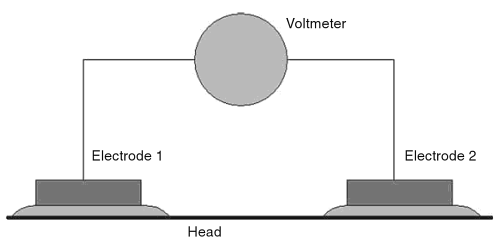
\includegraphics[width=0.70\textwidth]{voltmeter.png}
	\caption{Electrodes connected to a voltmeter~\cite[p.~120]{ERP}}
	\label{fig:voltmeter}
\end{figure}

Usually electrodes are placed on the scalp according to international 10-20 electrode location system. The outer layer of the brain can be classified into four lobes: temporal, occipital, parietal and frontal. See figure~\ref{fig:brain_lobes} for example. 10-20 electrode location system uses a letter and a number to identify electrode location. The letter is the first letter of the brain lobe above which the electrode is located and therefore the electrode measures the activity of this brain lobe. There are more complicated electrode-naming-systems that extend the 10-20 system. See figure~\ref{fig:electrode_locations} for illustration.

In a broad sense, \gls{EEG} recording is linked to the general state of the brain~\cite{VEP}. Therefore, due to the generality of the recording, potentials evoked by certain events cannot be seen in the recording because the evoked potentials are much smaller than the general fluctuations. A brain potential evoked by some event is called \gls{ERP}. 

\glspl{ERP} are linked to the information flow in the brain and are usually recorded by using an averaging technique~\cite{ERP}. For example, \glspl{ERP} can be recorded by presenting a stimulus with a certain time interval to a subject and calculating the average of \gls{EEG} signals recorded in the same time interval. This technique can be used because the stimuli is presented at a constant rate and thus \glspl{ERP} are also evoked one after another in the same constant interval. Therefore, \glspl{ERP} are always evoked at the same time while other fluctuations and noise are mostly random. When calculating the average of the \gls{EEG} recordings divided into the same time intervals as the stimulus presentation, the result will be an \gls{ERP} because other fluctuations and noise mostly cancel out in the averaging process. Thus \gls{EEG} can be used to record \glspl{ERP} from the scalp. 

\section{Visual evoked potential}
\label{sec:VEP}

In section~\ref{sec:EEG} brain potential called \gls{ERP} was discussed and it was noted that \glspl{ERP} are evoked by some event. The aim of this section is to describe \gls{ERP} called \gls{VEP} and discuss how \glspl{VEP} can be measured. As the name suggests, \glspl{VEP} are elicited by visual stimuli. The visual stimulus for eliciting a \gls{VEP} can be very simple, for example a white square blinking on a black computer screen.

When the visual stimulus is seen, the signal travels from the eyes to the \gls{visual processing centre} through the \gls{primary visual pathway} in the brain~\cite{neuroscience}. The \gls{visual processing centre} is located in the back of the brain. As mentioned in section~\ref{sec:EEG}, the outer layer of the brain can be classified into four lobes. The \gls{visual processing centre} is located in the occipital lobe. See figure~\ref{fig:lobes_pathway} for illustration. The \gls{primary visual pathway} is a \gls{neural pathway}; \glspl{neural pathway} were also mentioned in the section~\ref{sec:neuron}.

\begin{figure}[t]
	\centering
	\begin{subfigure}{0.48\textwidth}
		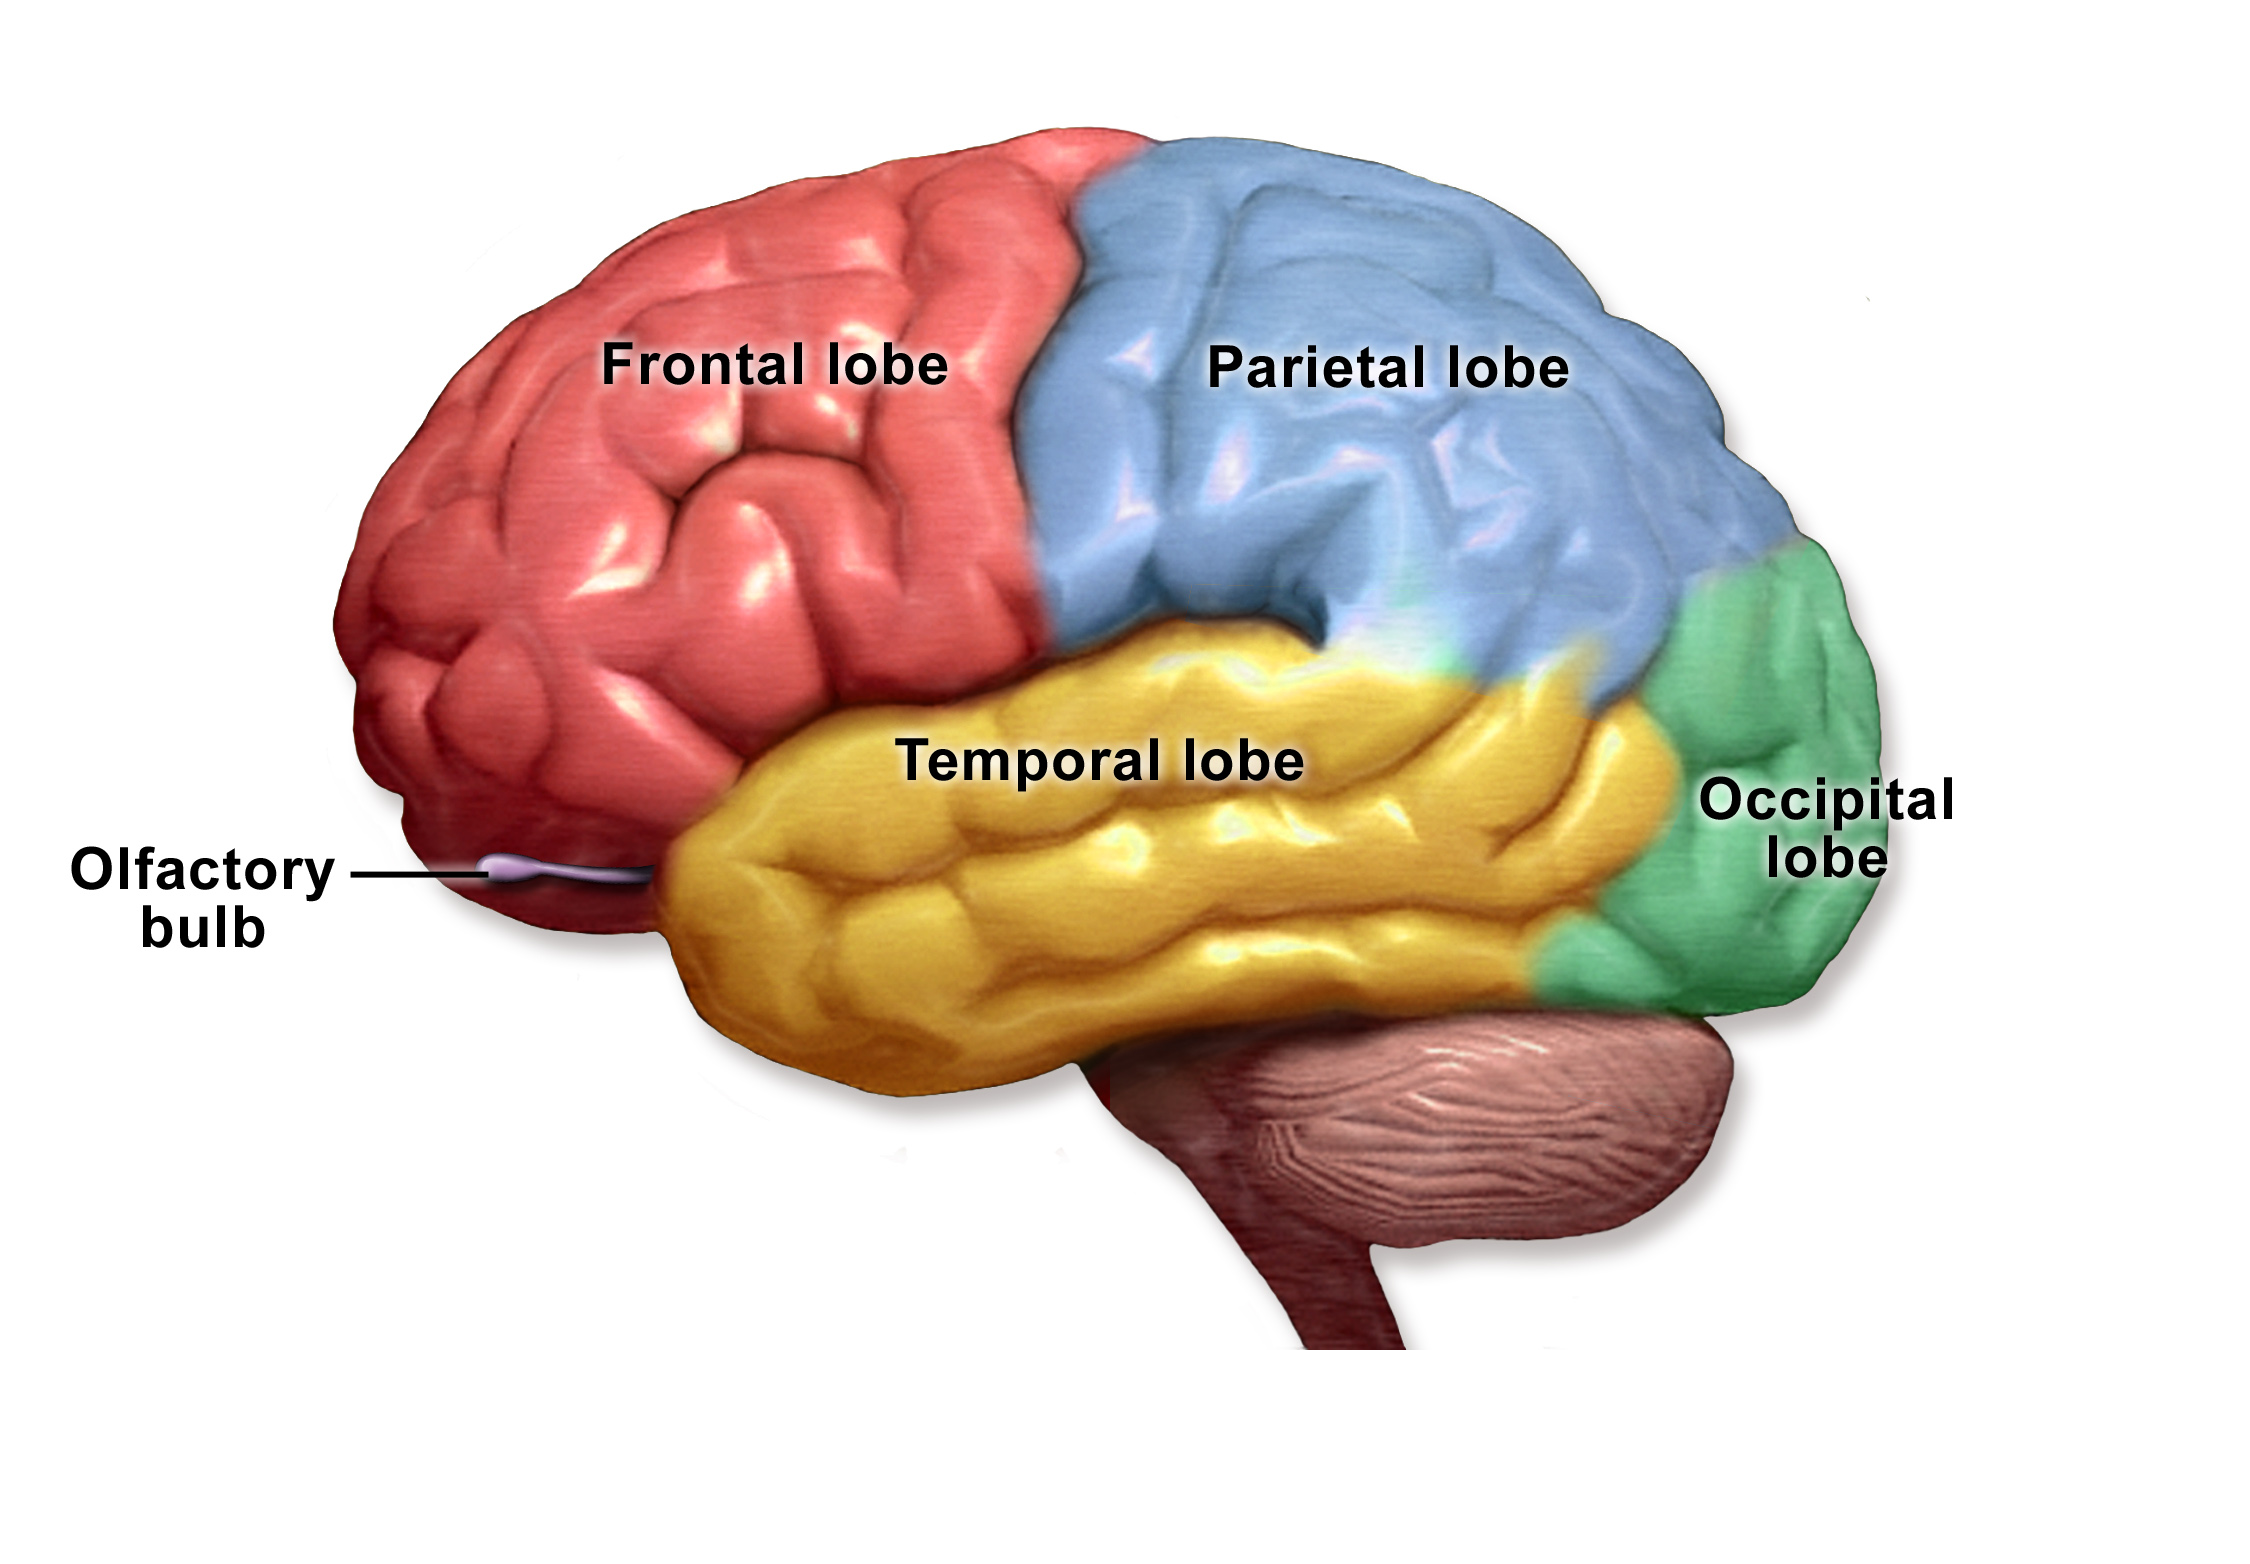
\includegraphics[width=\textwidth]{brain_lobes.png}
		\caption{Lobes of the brain~\cite{blausen}}
		\label{fig:brain_lobes}
	\end{subfigure}
	~
	\begin{subfigure}{0.48\textwidth}
		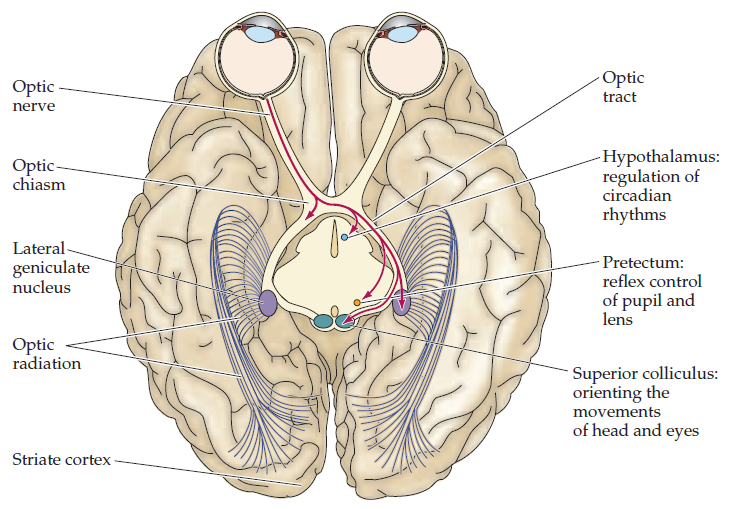
\includegraphics[width=\textwidth]{visual_pathway.png}
		\caption{The primary visual pathway~\cite[p.~261]{neuroscience}}
		\label{fig:visual_pathway}
	\end{subfigure}
	\caption{The location of occipital lobe and the neural pathway from eyes to the lobe}
	\label{fig:lobes_pathway}
\end{figure}

Due to the posterior location of the occipital lobe, electrodes must be placed to the back of the head when recording \glspl{VEP} with \gls{EEG}. These electrode locations are identified with the letter O as discussed in section~\ref{sec:EEG}.

When comparing the \glspl{VEP} elicited by
\begin{enumerate*}[(1)]
	\item the stimulation of the \gls{central visual field} and
	\item the stimulation of the \gls{peripheral vision}
\end{enumerate*} by the same stimuli, it can be seen that the stimulation of the \gls{central visual field} produces larger \glspl{VEP}~\cite{VEP_size}. In other words, the stimulus which a subject is looking at elicits larger \glspl{VEP} than those stimuli that are not in the very centre of gaze. Therefore, it is possible to present multiple visual stimuli to a subject and detect which stimulus is the subject looking at. 

To make the detection of \glspl{VEP} easier, \glspl{SSVEP} are used. If the visual stimulus is presented at a constant rate and the rate is so fast that the visual pathway does not have enough time to fully recover between stimulus presentations, then the elicited response becomes continuous and it is called the \gls{SSVEP}~\cite{VEP}. In a broad sense, \gls{SSVEP} is composed of many \glspl{VEP} that are elicited one after another in certain rate. See figure X for an example of \gls{VEP} and \gls{SSVEP}.

\gls{SSVEP} is continuous and therefore it is easier to detect it in the \gls{EEG} recording than \gls{VEP}, which is not continuous. Detecting continuous response is easier and more efficient because it is always present in the recording. Therefore, only \gls{SSVEP}-based methods used to detect \gls{SSVEP} in \gls{EEG} recording are discussed in this thesis.

%Thus the kind of response that is elicited in the brain depends on the visual stimulus. 

%\gls{SSVEP} reflects certain properties of the visual stimuli. Most important of these properties is that the %\gls{SSVEP} component frequencies depend on the frequency of the visual stimulus. the visual stimuli that are used to elicit \glspl{SSVEP} are discussed in section~\ref{sec:stimuli}.

%In conclusion, it is not efficient to detect \gls{VEP} itself in the \gls{EEG} recording and thus \gls{SSVEP} is used instead. 

%Research has shown that \gls{SSVEP} reflects certain properties of the visual stimulus. The visual stimuli that is used to elicit \gls{SSVEP} are further discussed in section~\ref{sec:stimuli}.  %The \gls{SSVEP} is composed of components that have different frequencies. The visual stimuli and signal components are further discussed in section~\ref{sec:stimuli} and section~\ref{sec:fourier} respectively. The frequency of the component that has the highest amplitude is the same as the \gls{fundamental frequency} or the lowest frequency of the visual stimulus. Thus \gls{SSVEP} can be detected in \gls{EEG} recording by finding and analysing the components of \gls{SSVEP} in the recording.
%The frequency of \gls{SSVEP} elicited by a visual stimulus is the same as the presentation rate or \gls{flickering} frequency of the visual stimulus. Furthermore, not only the frequency of the visual stimulus can be detected in the \gls{EEG} recording, but also its \glspl{harmonic}. \Glspl{harmonic} are components of \gls{SSVEP} that have frequency which is integer multiple of the fundamental frequency. Thus \gls{SSVEP} is composed of components each of which has frequency that is integer multiple of the lowest frequency in \gls{SSVEP}.

\section{Emotiv EPOC}
\label{sec:EEG_comparison}

In section~\ref{sec:neuroimaging} different functional neuroimaging methods were compared and it was concluded that currently \gls{EEG} is most suitable for designing inexpensive and portable interface for controlling a robot. But there is a wide variety of EEG devices available. The aim of this section is to briefly compare some of the devices and choose inexpensive and portable device available to the consumer.

Continuous signal cannot be directly represented in computers or in other digital devices and therefore continuous signal has to be converted to discrete signal to process it with a computer. As already mentioned in section~\ref{sec:EEG}, \gls{EEG} measures brain activity as function of voltage versus time. This function represents discrete signal, which means that both voltage and time are discrete. In other words, there is a finite set of possible values that the voltage can have and these values are acquired one after another in a certain rate. This rate at which digital values are extracted from a continuous signal is called \gls{sampling rate}. The device which converts continuous voltage to a sequence of discrete values is called \gls{ADC} device. \gls{ADC} resolution shows how many different values the device can represent.

The table~\ref{tab:EEG} shows comparison of different \gls{EEG} devices. Devices are compared by price, the number of electrodes or channels, the \gls{sampling rate} and the \gls{ADC} resolution. The higher the sampling rate, the more values are extracted in same time interval. The higher the \gls{ADC} resolution, the more different voltages the device can represent.

\newcommand{\patiCHamp}{\tablefootnote{http://www.brainvision.com/files/actiCHamp-PyCorder-Flyer\_US.pdf}}
\newcommand{\pmitsar}{\tablefootnote{http://www.novatecheeg.com/products--software.html}}
\newcommand{\pemotiv}{\tablefootnote{https://emotiv.com/epoc.php}}
\newcommand{\pmindwave}{\tablefootnote{http://store.neurosky.com/products/mindwave-1}}
\newcommand{\mitsarspec}{\tablefootnote{http://www.mitsar-medical.com/eeg-machine/eeg-amplifier-compare/}}
\newcommand{\popenbci}{\tablefootnote{http://openbci.myshopify.com/products/openbci-8-bit-board-kit}}

\begin{table}[h]
	\centering
	\begin{tabular}{|c|c|c|c|c|}\hline
								& Price						& Channels	& Sampling rate	& \gls{ADC} resolution	\\\hline
		Mindwave\pmindwave		& \SI{80}[\$]				& 1			& \SI{512}{Hz}	& 12 bit				\\\hline
		Emotiv EPOC\pemotiv		& \SI{400}[\$]				& 14+2		& \SI{128}{Hz}	& 16 bit				\\\hline
		OpenBCI\popenbci		& \SI{450}[\$]				& 8			& adjustable	& 24 bit				\\\hline
		Mitsar 202\mitsarspec	& \SI{10500}[\$]\pmitsar	& 31+1		& \SI{2}{kHz}	& 24 bit				\\\hline
		atiCHamp\patiCHamp		& \SI{77100}[\$]			& 160		& \SI{25}{kHZ}	& 24 bit				\\\hline
	\end{tabular}
	\caption{Comparison of EEG devices}
	\label{tab:EEG}
\end{table}

From the more consumer-friendly devices, Emotiv EPOC seems to offer good price-quality relationship. Furthermore, Emotiv EPOC is wireless. Emotiv EPOC has 16 electrodes, two of which are reference electrodes. Reference electrodes have two different possible locations: P3 and P4 or locations behind the ears. Other electrodes have fixed locations: AF3, AF4, F3, F4, F7, F8, FC5, FC6, P7, P8, T7, T8, O1, O2. See figure~\ref{fig:electrode_locations} for illustration. Emotiv EPOC has a sampling rate of \SI{128}{Hz}, an internal sampling rate of \SI{2048}{Hz} and an \gls{ADC} resolution of 16 bit. High internal \gls{sampling rate} is used to remove high frequency artefacts from the signal. The signal is filtered and transmitted to wireless receiver with reduced \gls{sampling rate} of \SI{128}{Hz}.

\begin{figure}[h]
	\centering
	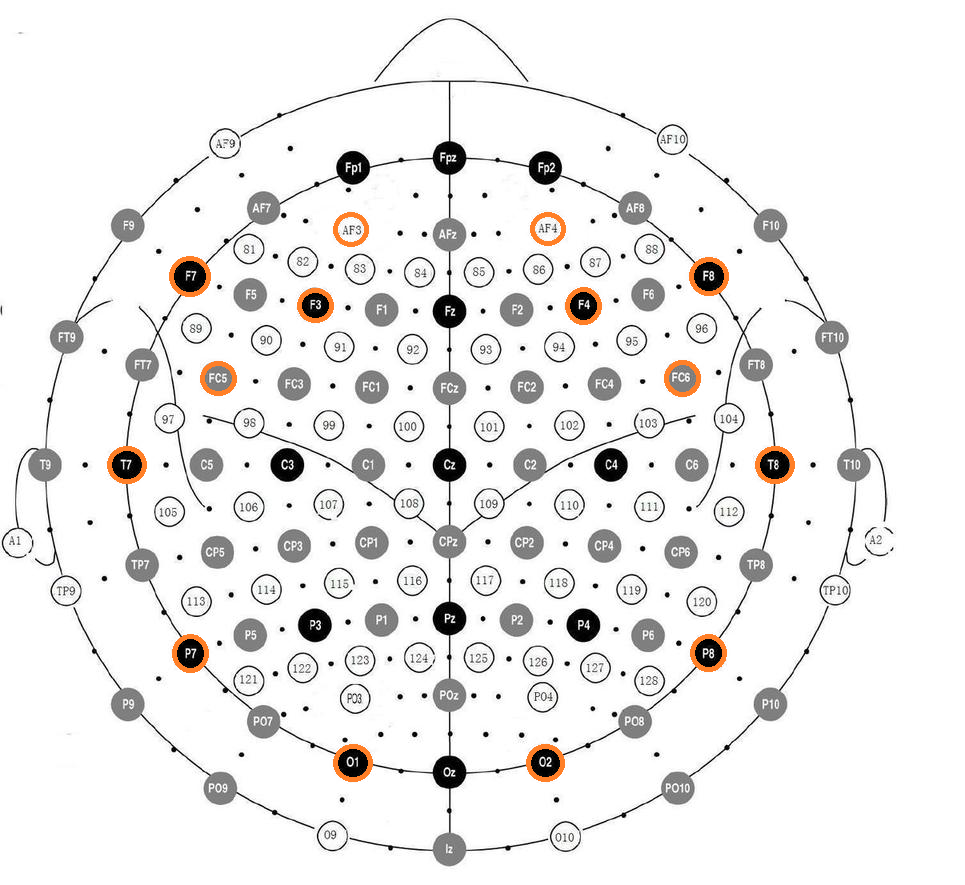
\includegraphics[width=0.8\textwidth]{electrode_locations.png}
	\caption{Electrode locations used by Emotiv EPOC\protect\footnotemark}
	\label{fig:electrode_locations}
\end{figure}

Research has shown that Emotiv EPOC performs significantly worse than a medical-grade device~\cite{emotiv_p300_comp}. But the performance of Emotiv EPOC is good enough to detect \glspl{SSVEP} in the recording~\cite{emotiv_11hz, emotiv_psda, emotiv_walking, emotiv_comparison}. It has also been shown that it is possible to use Emotiv EPOC even when the subject is walking during recording~\cite{emotiv_walking}. Walking during the recording session causes the device to move and this movement produces artefacts in the recording. Despite the artefacts in the recording, it is still possible to detect \glspl{SSVEP} in the recording. Thus the performance of Emotiv EPOC is sufficient for detecting \glspl{SSVEP} and it is chosen as \gls{EEG} device for controlling a robot in this thesis.
\footnotetext{http://emotiv.wikia.com/wiki/Emotiv\_EPOC}
